\documentclass{article}
\usepackage{graphicx}

\title{Coin Change}
\author{William Y. Feng}

\begin{document}

\maketitle
You just moved to the UK last week, and, needing to provide a living for yourself, you found a job as a cashier at a large retail store in central London. Today's your first day on the job—you're a little nervous, mostly about rude customers, but are excited to do the job nonetheless.

The first customer of the day walks to your checkout line and hands you a calculator. You scan it, run the totals, and it comes out to $\pounds 9.60$. The customer pays with a ten-pound note, so you'll need to give them back 40 pence in change.
\begin{center}
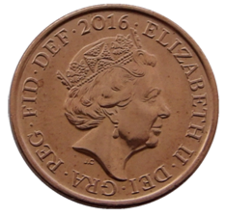
\includegraphics[scale=0.6]{images/british_coin.png}
\end{center}
Seems simple enough; the cash register pops open and you discover \textit{six coin denominations}: \textit{1p} \textit{p is short for pence}, \textit{2p}, \textit{5p}, \textit{10p}, \textit{20p}, and \textit{25p}.

Making 40 pence should be a breeze. You use a \textit{greedy algorithm} and start by taking a 25p coin, leaving 15p to make—so you finish with a 10p and a 5p. You collect these three coins and hand them to the customer.

"Wait," they say. "I'll excuse you, since I can tell you're probably an American and it looks like you're new on the job—but there's a more efficient way to make 40 pence."

You're confused. You just went through the coin denominations in decreasing order, and 25p, 10p, and 5p seems like a pretty optimal way to make 40p change.

"You could have just given me two 20p coins."

The realization hits you with the weight of a train. How did your greedy algorithm fail? Is using up large-denomination coins first not the optimal way to make change to minimize the number of coins? The customer's remark shakes the very foundations of your understanding of currency. Maybe you weren't made out to be a cashier in the UK after all.

\begin{center}
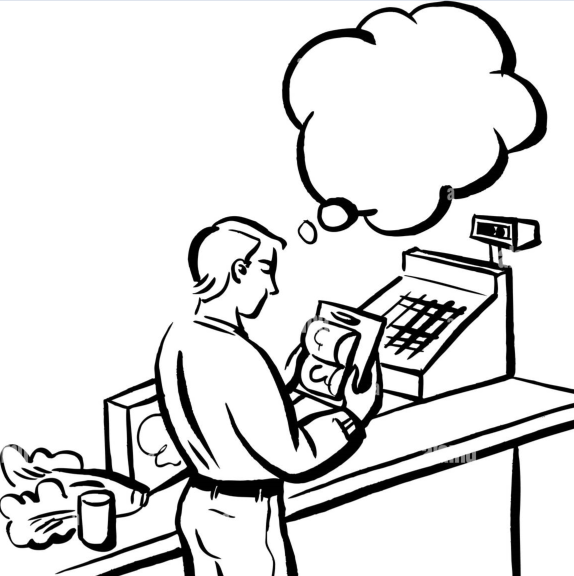
\includegraphics[scale=0.6]{Magazines/img/Vol4/cashier.jpg}
\end{center}

"It's okay, you don't get the same problem in America. And we don't usually get this in the UK either; we can prove that it's because of those commemorative 25p coins that your greedy algorithm didn't work."

This customer must be either a genius or a mathematician. You're interested in hearing more; perhaps this person can rebuild some of your foundations of mathematics that they just violently tore down.

"Here's a simpler example: suppose we have to make 10 pence with only 1-pence, 3-pence, and 4-pence coins. What's the minimum number of coins we must use?"

You're hesitant to reply, because this customer has just made you so unsure of yourself. The greedy approach would have you use as many 4p coins as possible first, then 3p coins, then 1p coins. This would result in using two 4p coins and two 1p coins to make 10p.

"Surely there's a more optimal way than being greedy here," you say. "I can use four coins—two 4p and two 1p—to make 10p, but we can probably do better."

"You're exactly right," says the customer. "Consider this: to make 10 pence, we have three options:
\begin{enumerate}
\item Take a 4p coin, and make the remaining 6p optimally
\item Take a 3p coin, and make the remaining 7p optimally
\item Take a 1p coin, and make the remaining 9p optimally
\end{enumerate}
In other words, if we define the following function:
$C(n) = \text{minimum number of coins to make n pence}$
then we can write
\[
C(n) = \text{minimum of }
\begin{cases}
    1 + C(n - 4) \\
    1 + C(n - 3) \\
    1 + C(n - 1)
\end{cases}
\]
Each of those three cases is one potential universe of possibilities, and we want the one which uses the minimum number of coins. This function only works in this specific scenario—we'd have to modify it if we wanted to use, say, British coin denominations."

"That's an interesting way of framing this problem. How can we actually compute $C(n)$, though?" you reply.

"Good question! We can do it by iteratively finding $C(i)$ for all the $i$ less than $n$. Suppose we want to calculate $C(10)$, and already have all the values of $C(1), C(2), \dots, C(9)$.

\begin{table}[h]
    \centering
    \begin{tabular}{c|c|c|c|c|c|c|c|c|c|c}
        $n$ & 1 & 2 & 3 & 4 & 5 & 6 & 7 & 8 & 9 & 10 \\\hline
        $C(n)$ & 1 & 2 & 1 & 1 & 2 & 2 & 2 & 2 & 3 & 
    \end{tabular}
\end{table}
To fill out the entry for $C(n)$, we consider each of those three possibilities.
\begin{enumerate}
    \item What if we used a 4p coin? Then we'd have 6p left, which we \textit{know for sure} is optimally constructed with $C(6) = 2$ coins. Adding on the 4p coin, this makes 3 coins in total.

    \item There are other ways—if we used a 3p coin, then we'd have 7p left, which we know can be optimally constructed with $C(7) = 2$ coins, giving the possibility to construct 10p with 3 coins yet again.

    \item And if we used a 1p coin, then we'd have 9p left, which we know is optimally constructible with $C(9) = 3$ coins, making 4 coins total.
\end{enumerate}

Thus we have three alternatives, and we take the best one. In this case, either of the first two work, so $C(10)$ should be 4. We could even keep going if we wanted to; now that we have the first 10 values of $C(n)$, we can find $C(11)$, then $C(12)$, and so on."

Fascinating! This customer has just given you an incredibly fast way to determine the minimum number of coins to make any arbitrary amount of change.

"And you said this works for British denominations, too?" you ask.

"Why, of course—the function would just look something like this instead:
\[
C(n) = \text{minimum of }
\begin{cases}
    1 + C(n - 25) \\
    1 + C(n - 20) \\
    1 + C(n - 10) \\
    1 + C(n - 5) \\
    1 + C(n - 1)
\end{cases}
\]
This technique works for any denomination imaginable."

% It's starting to feel like you're a character in a contrived story about coin-change making methods.

You hear a shout from the back of the queue. While this person's been teaching you about optimal coin change-making methods, many more customers have arrived.

"Blimey, what's taking so long up there? This is supposed to be the ten-items max queue."

You turn back to the customer and confidently hand this customer two twenty-pence coins, grateful that they have given you such a valuable lesson.
\end{document}